%Matteo Kumar - Leonard Schatt
% Fortgeschrittenes Physikalisches Praktikum
% Main-Datei für die Auswertung in TeX

% Struktur:
% Für jeden Abschnitt gibt es einen Ordner, damit jeder individuell an seinen Aufgaben arbeiten
% kann, ohne beim merge in GitHub Konflikte zu erhalten. Deshalb werden alle Unteraufgaben auch 
% extra in Ordner angelegt. Die einzelnen Dateien über den input Befehl einfügbar.
% Bilder und andere Grafik werden im Ordner Grafik abgelegt 


% Packages
\documentclass[paper=a4,bibliography=totoc,BCOR=10mm,twoside,numbers=noenddot,fontsize=11pt]{scrreprt}
\usepackage[ngerman]{babel}
\usepackage[latin1, utf8]{inputenc}
\usepackage[babel,german=quotes]{csquotes} %For Quotes
\usepackage[T1]{fontenc}
\usepackage{lmodern}
\usepackage{graphicx}
\usepackage{nicefrac}
\usepackage{fancyvrb}
\usepackage{amsmath,amssymb,amstext}
\usepackage{siunitx}
\usepackage{url}
\usepackage{natbib}
\usepackage{microtype}
\usepackage[format=plain]{caption}
\usepackage{physics}
\usepackage{titleref}

% Zusätzliche Packages
\usepackage{geometry}
\usepackage{anyfontsize}
\usepackage[table]{xcolor}
\usepackage{ifthen}
\usepackage[absolute,overlay]{textpos}
\usepackage{amsfonts}
\usepackage{xstring}
\usepackage{tikz}
\usepackage{pdfpages}
\usepackage{booktabs}
\usepackage{hyperref}

% Abschnittseinrückung und -abstand
% Die folgenden Zeilen sollen möglichst nicht verändert werden
\parindent 0.0cm
\parskip 0.8ex plus 0.5ex minus 0.5ex

% Anzahl und Größe von Gleitobjekten
% maximal 2 Objekte oben und unten
% erlaubt auch größere Bilder, welche die ganze Seite benötigen
% Die folgenden Zeilen sollen möglichst nicht verändert werden
\setcounter{bottomnumber}{2}
\setcounter{topnumber}{2}
\renewcommand{\bottomfraction}{1.}
\renewcommand{\topfraction}{1.}
\renewcommand{\textfraction}{0.}

%\sc und \bc veraltet. Daher: (20.09.2018)
\DeclareOldFontCommand{\sc}{\normalfont\scshape}{\@nomath\sc}
\DeclareOldFontCommand{\bf}{\normalfont\scshape}{\textbf}

% Verschiedenes
\pagestyle{headings}          % Der Seitenstil sollte möglichst nicht verändert werden
\graphicspath{{./bilder/}}    % Der Pfad für die Abbildungen Abbildungen wird gesetzt
\VerbatimFootnotes            % \verb etc.

% Funktionen
\newcommand\tab[1][1cm]{\hspace*{#1}}
\newcommand{\vect}[1]{\boldsymbol{\mathbf{#1}}}
\newcolumntype{g}{>{\columncolor[rgb]{ .741,  .843,  .933}}l}
\DeclareSIUnit\angstrom{\text{\AA}}
\pgfplotsset{compat=1.18}

\begin{document}

    \nonfrenchspacing

    % 0. Kapitel 
    %Matteo Kumar - Leonard Schatt
% Fortgeschrittenes Physikalisches Praktikum
% 0. Cover
% Noch abänderbar nur ein Vorschlag
\newgeometry{top=30mm, bottom=20mm, inner=20mm, outer=20mm}
\thispagestyle{empty}

% Colors
\definecolor{Notablue}{HTML}{3498DB}		%Theoretische Physik
\definecolor{Notared}{HTML}{CF366C}			%Mathematik
\definecolor{Notagreen}{HTML}{19B092}		%Experimentalphysik
\definecolor{Notaorange}{HTML}{FA9D00}		%Chemie/Wahlfach nicht physikalisch
\definecolor{Notagrey}{HTML}{969696}		%Praktikum
\definecolor{Notalavendel}{HTML}{9DBBD8}	%Wahlfächer physikalisch

% Boolean by default false
\newboolean{twoRows}
\newboolean{symbol}

% Funktions
\makeatletter
   \def\vhrulefill#1{\leavevmode\leaders\hrule\@height#1\hfill \kern\z@}
\makeatother
\newcommand*\ruleline[1]{\par\noindent\raisebox{.8ex}{\makebox[\linewidth]{\vhrulefill{\linethickness}\hspace{1ex}\raisebox{-.8ex}{#1}\hspace{1ex}\vhrulefill{\linethickness}}}}

% Variables
\def\schriftgrosse{70}
\def\linethickness{1,5pt}

\def\farbe{Notagrey}
\def\fach{PPD}
\def\name{Matteo Kumar - Leonhard Schatt}
\def\uberschrift{Lightsheet Microscopy} % Absatz mit \\[0,5cm]; u = Übung, k = Klausur; s = Skript, e = Ergebnis
\def\bottom{SS 2023}
\def\datum{03.07.23}
\def\platz{}
\def\betreuer{Ivana Jeremic}
\def\groupnr{2}

\begin{titlepage}
			
	\centering
	{\LARGE \sffamily {\textbf{\bottom}\par}}
	\vspace{2,5cm}
    {\fontsize{40}{0}\sffamily\ruleline{\textcolor{\farbe}{\textbf{\fach}}}\par}
    \vspace{6cm}
	{\Large\sffamily \ruleline{\name}\par}
	
	
	% Choose Text
	\ifthenelse{\equal{\uberschrift}{s}} {\def\titel{Skript}}	
		{\ifthenelse{\equal{\uberschrift}{k}} {\def\titel{Klausur}}
			{\ifthenelse{\equal{\uberschrift}{u}} {\def\titel{Übung}}
				{\ifthenelse{\equal{\uberschrift}{e}} {\def\titel{Klausur \\[0,5cm] Ergebnis}}
					{\def\titel{\uberschrift}}
				}
			}
		}
	
	\begin{textblock*}{21cm}(0cm,9cm) % {block width} (coords), centered		
		{\fontsize{\schriftgrosse}{0}\sffamily\textcolor{\farbe}{\textbf{\titel}}\par}
	\end{textblock*}
	
	% Choose Logo
	\ifthenelse {\equal{\farbe}{Notared}} {\def\logo{Bilder/Logo/UniBTNotared}}
		{\ifthenelse {\equal{\farbe}{Notagreen}} {\def\logo{Bilder/Logo/UniBTNotagreen}}
			{\ifthenelse {\equal{\farbe}{Notablue}} {\def\logo{Bilder/Logo/UniBTNotablue}}
				{\ifthenelse {\equal{\farbe}{Notaorange}} {\def\logo{Bilder/Logo/UniBTNotaorange}}
					{\ifthenelse {\equal{\farbe}{Notagrey}} {\def\logo{Bilder/Logo/UniBTNotagrey}}
						{\ifthenelse {\equal{\farbe}{Notalavendel}} {\def\logo{Bilder/Logo/UniBTNotalavendel}}	
							{\ifthenelse {\equal{\farbe}{black}} {\def\logo{Bilder/Logo/UniBT}}	
								{\def\logo{noLogo}}
							}
						}
					}
				}
			}
		}	

	\IfSubStr{\logo}{noLogo}{\setboolean{symbol}{false}}{\setboolean{symbol}{true}}
	
	% Gruppe
	\vspace{10cm}
	{\large\sffamily{Group \groupnr}}
	
	%Logo
	\vfill

	\ifthenelse{\boolean{symbol}}
		{
			\begin{figure}[h]
			\begin{center}
				
				\includegraphics[width=2cm]{\logo}
				
			\end{center}
			\end{figure}
		}
	
\end{titlepage}

\restoregeometry

% Information
\chapter*{General Information}
\label{chap:info}

\begin{tabular}{l l}

	{\textbf{Date}} \hspace{1cm} & \hspace{1cm} {\datum}\\[0,2cm]
	{\textbf{Supervisor}} \hspace{1cm} & \hspace{1cm} {\betreuer}\\[1,2cm]
	{\textbf{Group No.}} \hspace{1cm} & \hspace{1cm} {\groupnr}\\[0.2cm]
%	{\textbf{Auswertperson}} \hspace{1cm} & \hspace{1cm} {\auswertp}\\[0.2cm]
%	{\textbf{Messperson}} \hspace{1cm} & \hspace{1cm} {\messp}\\[0.2cm]
%	{\textbf{Protokollperson}} \hspace{1cm} & \hspace{1cm} {\protop}\\[0.2cm]

\end{tabular}

    \thispagestyle{empty}
    \cleardoublepage
    \tableofcontents
    \cleardoublepage

    % 1. Kapitel Einleitung
    %Matteo Kumar - Leonard Schatt
% Fortgeschrittenes Physikalisches Praktikum

% 1. Kapitel Einleitung

\chapter{Introduction}
\label{chap:einleitung}




    % 2.Kapitel Fragen zur Vorbereitung
    %Matteo Kumar - Leonard Schatt
% Fortgeschrittenes Physikalisches Praktikum
 
\chapter{Theorie}
\label{cha:theory}

This chapter discusses the theoretical basis for this laboratory practice.


    % 3.Kapitel Protokoll
    % Matteo Kumar, Leonard Schatt
% Physikalisches Praktikum


\chapter{Methods, setup and materials}
\label{chap:methods}

In this chapter the used setup, methods and materials are introduced.


\section{Film preparation}
\label{sec:FilmProd}

In the following section the film production is explained.

\subsection*{Substrate and solution production}

The following section explains how the sample substrate is produced.

As substrate glass slides are used. We cut those slides in rectangles of the dimension \SI[]{15}{mm} x \SI[]{25}{mm}. Afterwards the
glass slides were cleaned in the following liquids in the ultrasonic bath for 10 minutes and dried afterwards with nitrogen:

\begin{enumerate}
    \item Aqueous Alconox solution $0.16\,\frac{\mathrm{g}}{\mathrm{ml}}$
    \item Deionised water
    \item 2-Propanol
\end{enumerate}

The chlorobenzene and polystyrene solution used is prepared from a solution of \SI{300}{\milli\gram\per\milli\liter} by dilution. 
We produce approximately \SI{250}{\micro\liter} of solutions with the concentrations \SI{300}{\milli\gram\per\milli\liter}, \SI{250}{\milli\gram\per\milli\liter}, \SI{200}{\milli\gram\per\milli\liter},
\SI{150}{\milli\gram\per\milli\liter}, \SI{100}{\milli\gram\per\milli\liter}, \SI{50}{\milli\gram\per\milli\liter}, \SI{25}{\milli\gram\per\milli\liter} and \SI{1}{\milli\gram\per\milli\liter}.

\subsection*{Spincoating}

The films are produced using static spincoating.
In this method the solution is placed on the substrate. The spincoater is starting to spin the substrate. The centrifugal forces drive the solution away from the substrate.
This process enables the production of very homogeneous and thin layers.  

\begin{figure}[ht]
    \centering
    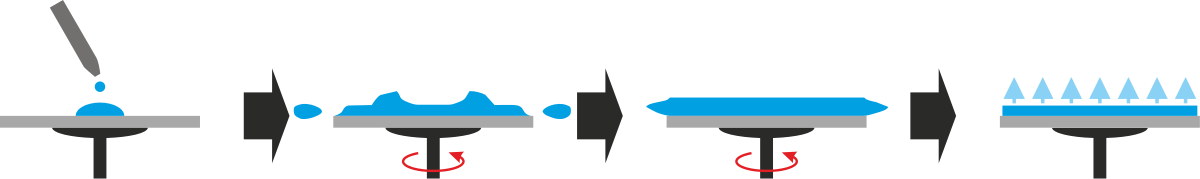
\includegraphics[width = \linewidth]{Bilder/Grundlagen/Spincoating.png}
    \caption[Graphical representation of the spincoating]{Graphical representation of the spincoating. From left to right, solution is placed in the substrate, the the coater spins and distributes the solution on the substrate. Afterwards the substrate drys.  From \textit{Stefan Reich \protect\footnotemark} }
    \label{fig:Spincoat}
\end{figure}

\footnotetext{(\url{https://commons.wikimedia.org/wiki/File:Spincoating.svg}), „Spincoating“, \url{https://creativecommons.org/publicdomain/zero/1.0/legalcode} }

We spincoat \SI{100}{\micro\litre} of the polymer solution onto the substrate.
The films for rotations dependence measurement were coated from a solution of \SI{100}{\milli\gram\per\milli\liter} at rotation rates of
\SI{500}{rpm}, \SI{750}{rpm}, \SI{1000}{rpm}, \SI{2000}{rpm}, \SI{3000}{rpm}, \SI{4000}{rpm} and \SI{5000}{rpm} for \SI{30}{\second}. This was done by \textit{Fabian Eller}.
Afterwards, a set of films is coated all with \SI{1000}{rpm} for \SI[]{90}{\second} but with all the above mentioned concentrations.
\section{Setup}
\label{sec:setup}

In the following, the setup is explained. 

The measurement setup comprises a broad-spectrum lamp and a UV-Vis spectrometer situated at the end of a light guide. This setup can be used for both reflectance and transmission measurements. To measure reflectance, a fiber with three ends is used, with inputs for the lamp and outputs for both the UV-Vis and NIR spectrometers (see Figure \ref{fig:setup}). On the other end of the fiber, there is a combination of input and output ends. The single end is positioned in the sample holder, with the sample placed at approximately 1 cm below sample holder.

\begin{figure}[ht]
    \centering
    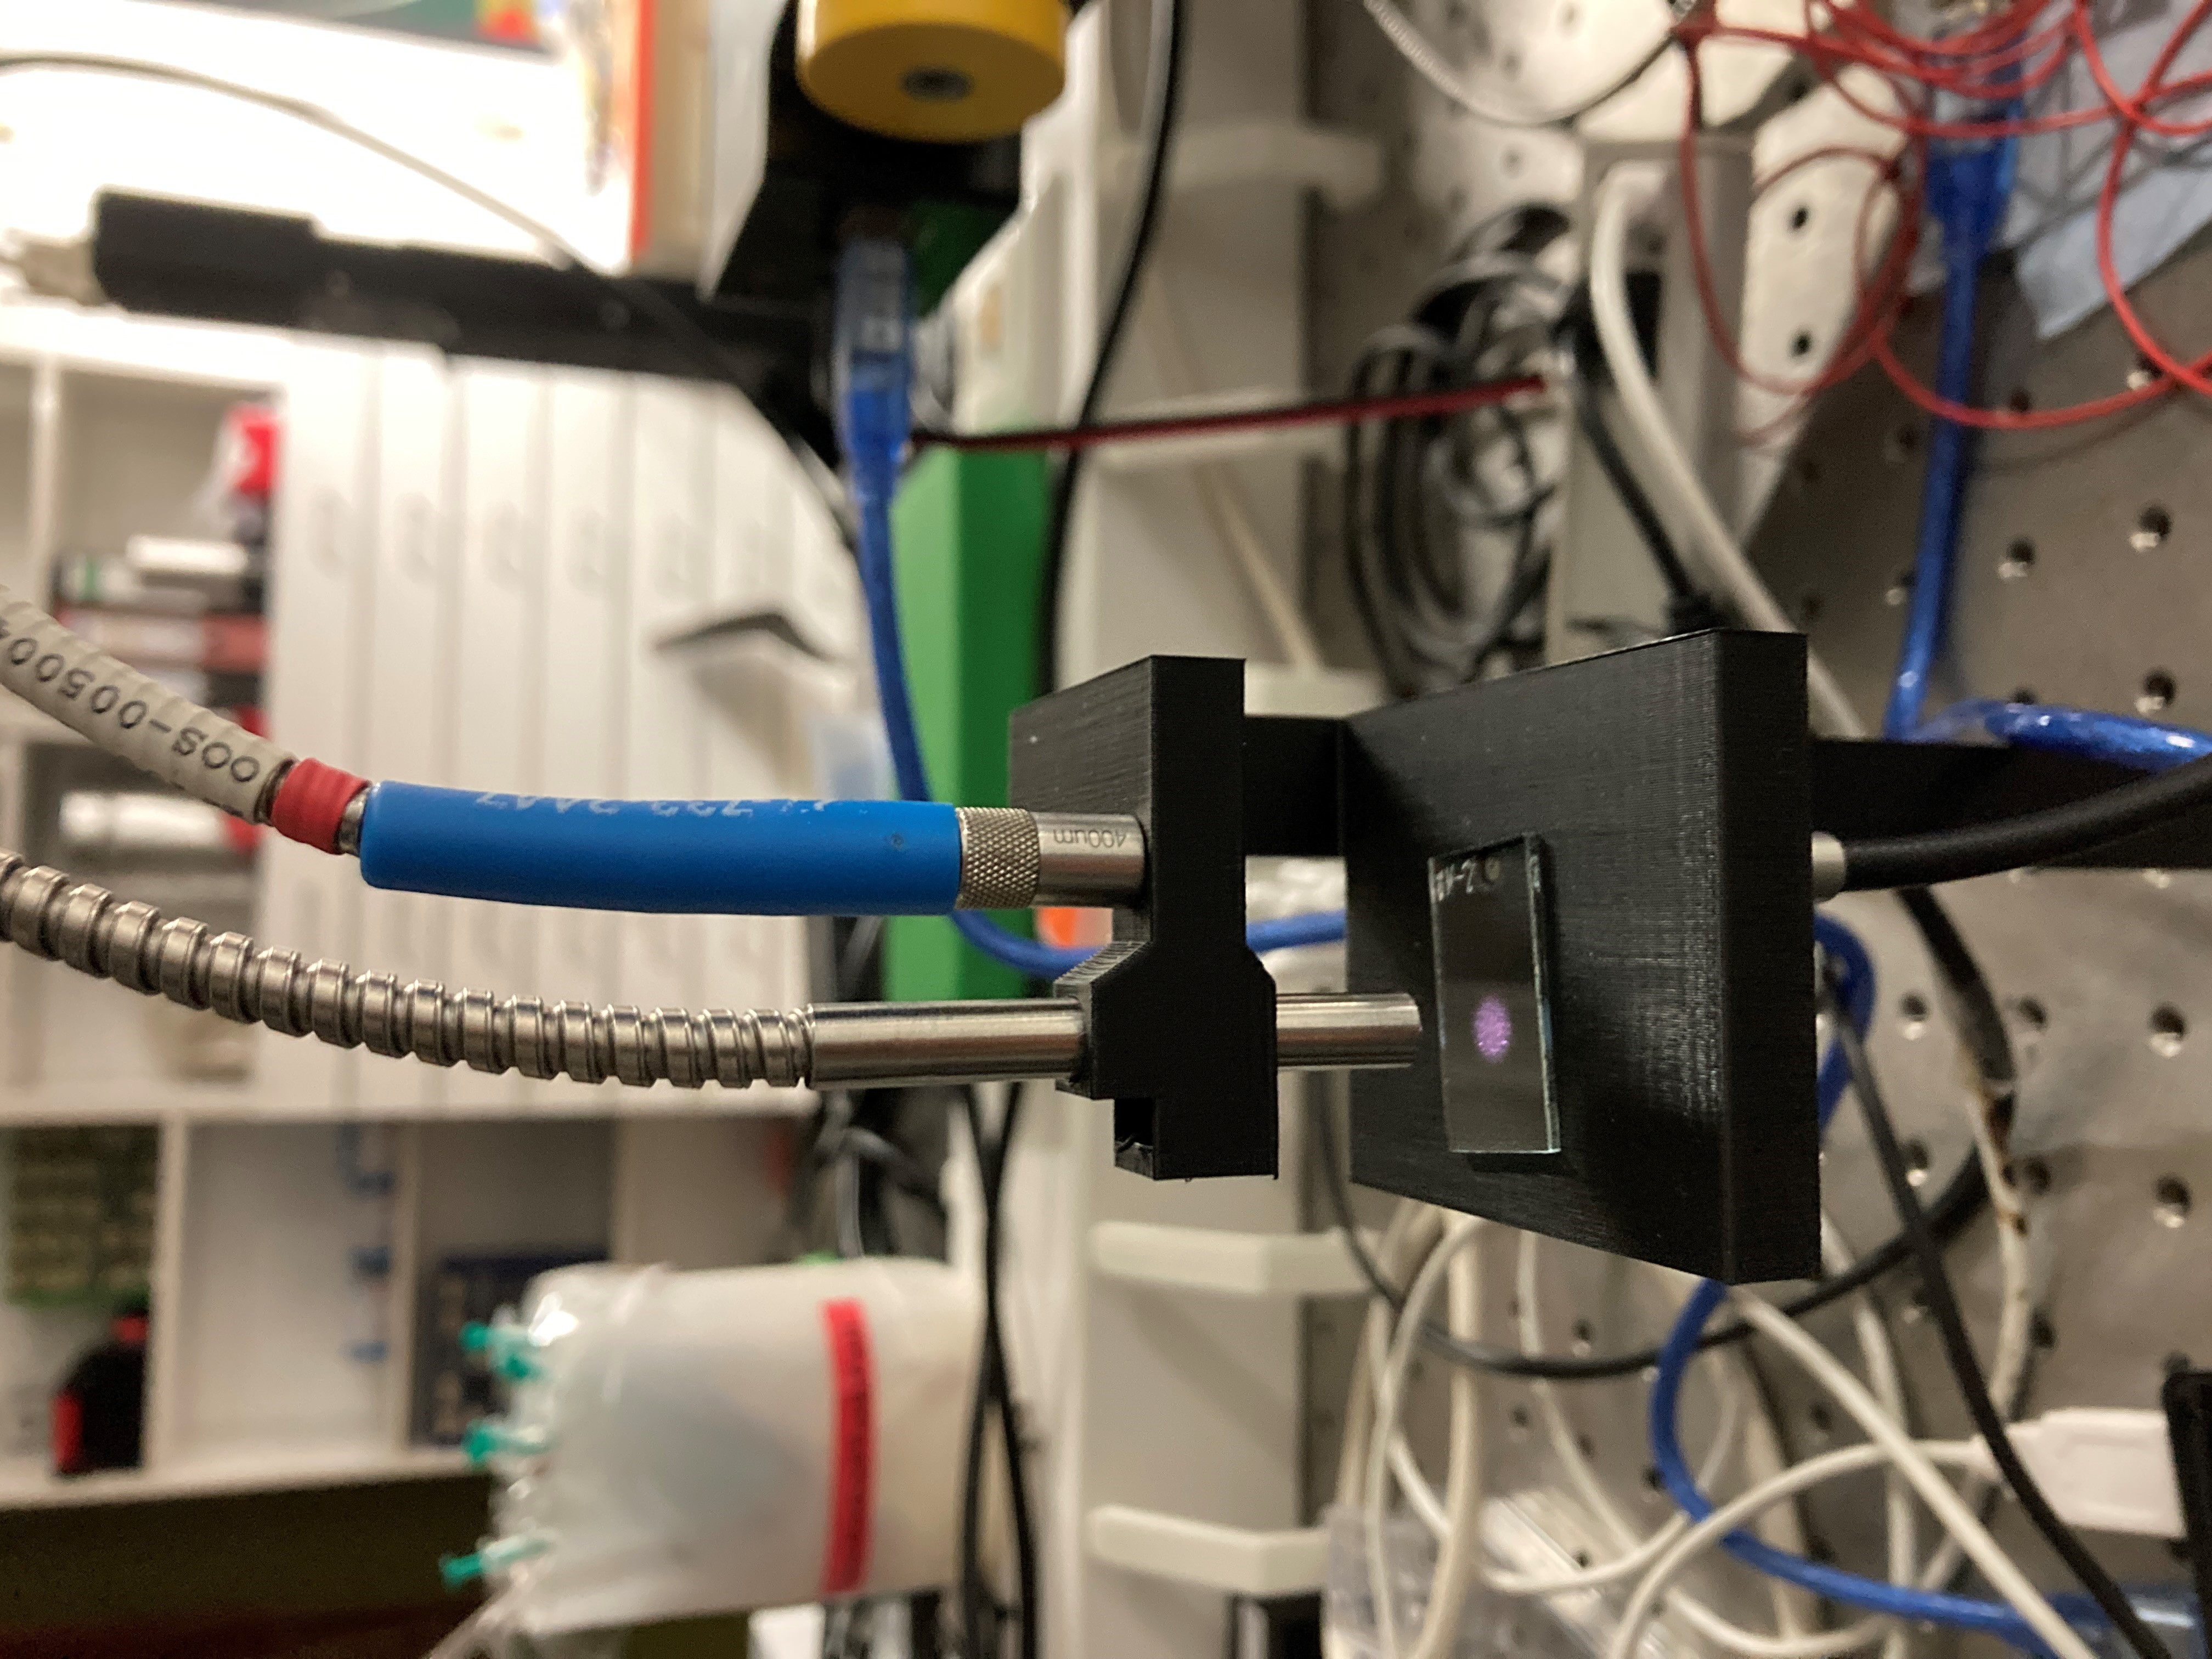
\includegraphics[width = 10cm]{Bilder/Auswertung/Setup/Setup.jpg}
    \caption{Sample holder with optic fiber and film}
    \label{fig:setup}
\end{figure}

Before conducting each series of film measurements, we capture a white spectrum of the lamp without any film. This data is then used by the program \textit{Nanocalc} to calculate the absorbance. At the start of each series, we measure the background once. Subsequently, we measure the spectrum of each film at six randomly selected points.

    % 4.Kapitel Versuchsauswertung
    % Matteo Kumar - Leonard Schatt
% Fortgeschrittenes Physikalisches Praktikum
% 4.Kapitel Versuchsauswertung

\chapter{Discussion}
\label{chap:versuchsauswertunDiscusion}

\section{Characterization of the light sheet}
\label{sec:LightSheet}


\section{Point spread function}
\label{sec:PSF}

In this section, we examine the point spread function (PSF) by studying a 3D stack of photos of beads that are
embedded in an agarose matrix. The matrix prevents the beads from moving. Since the beads are smaller
than the resolution, we can observe diffraction patterns. The diffraction pattern commonly observed for a spherical object is represented by an Airy function, which can be seen in \cref{fig:Airy}. 
Since the resolution is not sufficient to distinguish the secondary peaks from the main peak, they appear as shoulders.
\begin{figure}[h]
    \centering
    \begin{subfigure}{0.51\linewidth}
        \centering
        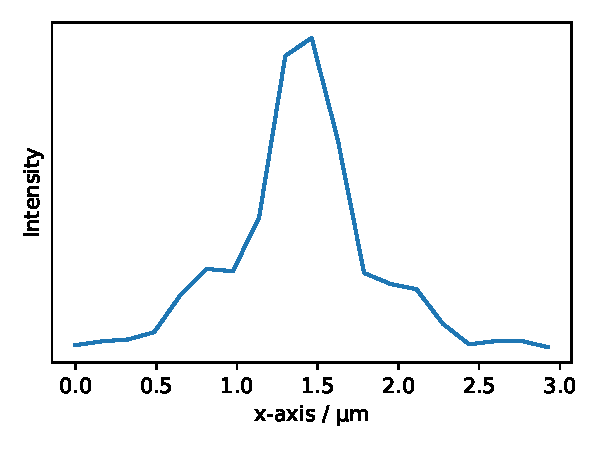
\includegraphics[width = \textwidth]{Bilder/PSF/Airy.pdf}
        \caption{Cut through the picture in \ref*{subfig:AiryBild}}
        \label{subfig:Airy}
    \end{subfigure}
    \hfill
    \begin{subfigure}{0.43\linewidth}
        \centering
        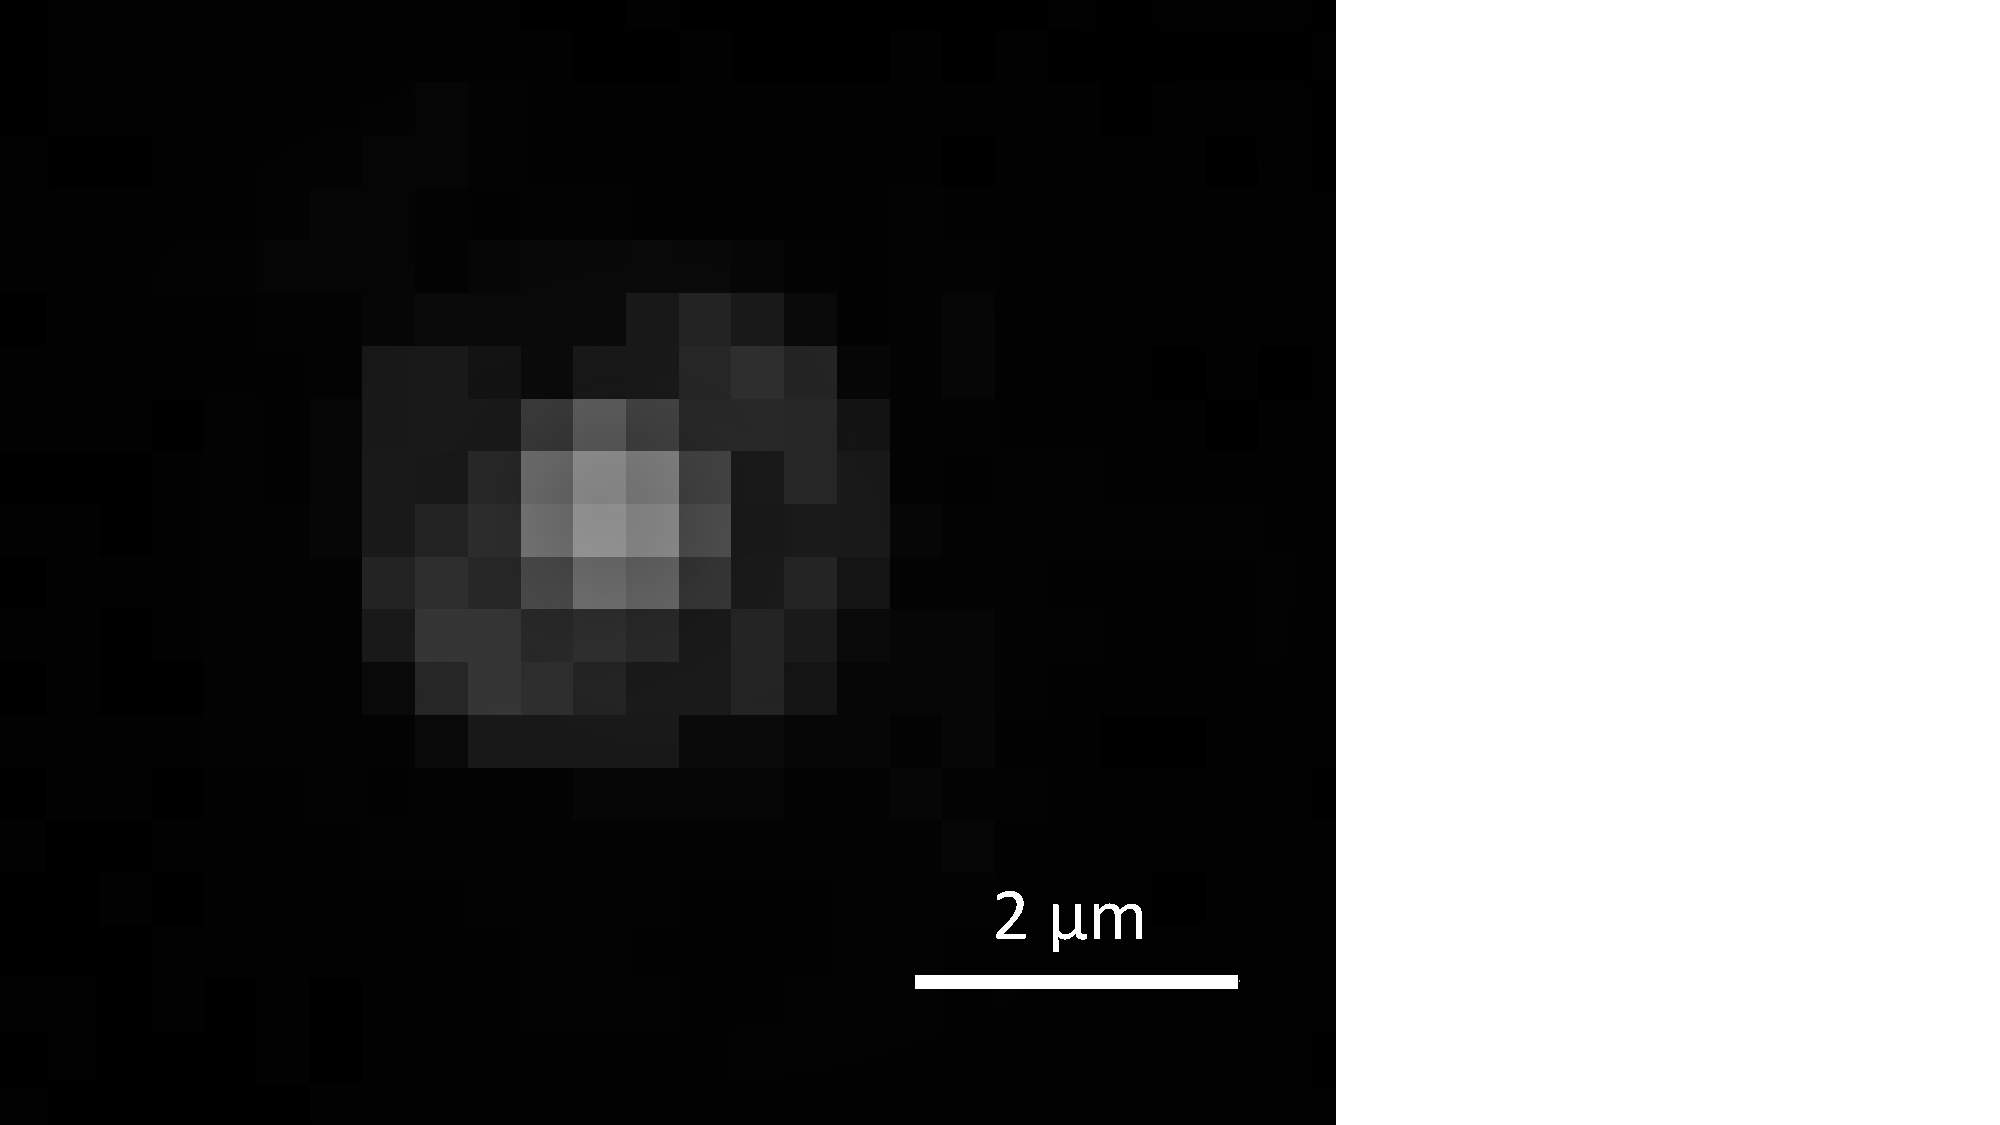
\includegraphics[width = \textwidth]{Bilder/PSF/2DBeugung_cropped.pdf}
        \caption{Image of a beat}
        \label{subfig:AiryBild}
    \end{subfigure}
    \caption{Image of a beat collected with a light sheet microscope (right) and a horizontal cut depicting the intensity profile (left). The intensity profile has one main peak and two separate smaller peaks, which appear as shoulders.}
    \label{fig:Airy}
\end{figure}


The particles were captured at four distinct locations (see \cref{fig:sites}) using no pinhole. Additionally, position 1 was imaged using both a half-open and a closed pinhole. Notably, the particles at positions 2 and 3 exhibited significant aberrations (see \cref{tab:FWHM}).
Conversely, the particles at positions 4 and 1 displayed small aberrations, which led to the selection of position 1 for subsequent measurements.


The FWHM is extracted using a Gaussian fit to the cuts, as shown in \cref{subfig:Airy}. The fitting is
performed using \textit{scipy.optimize.curve\_fit()}. Since the amount of available data does not allow
for its calculation, the uncertainty is not estimated. For each case, three beads in and out of
focus are analyzed. The results are presented in \cref{tab:FWHM}.

We encountered challenges in certain cases when identify to locate out-of-focus beads as there is no clear criteria to distinguish the two species.
Additionally, we experienced issues with the data from position 2. Our initial attempt to measure the stack of images was unsuccessful. 
Upon restarting the measurement, no beads were visible anymore. The images captured prior to the measurement failure depict heavily distorted beads, making them unsuitable for analysis using Gaussian fits.
Our reconstruction of the situation leads us to believe that we made the sample crash into the objective lens. This changes the optical properties of the objective lens because 
the refractive index difference is different. The force on the objective lens causes the programme to crash. Due to the impact, the sample was shifted out of focus. Therefore in the second measurement nothing is to be seen.
Furthermore, some interesting effects appear in the data. Certain patterns can be observed from time to time in our data. We do see for example 
some kind of smudged images as shown in \cref{fig:Verueckttebeats}. This look like the motor was from time to time not synchronized with the clock of the motor. 

\begin{table}[ht]
    \centering
    \begin{tabular}{cccc}
        \toprule Position 1: FWHM / $\SI{}{\micro \meter}$ & \textbf{x} &\textbf{y} & \textbf{z} \\
        \hline\hline open pinhole & $0.82\pm0.04$ & $0.84\pm0.04$ &  $3.1\pm0.4$ \\
        & \textcolor{gray}{$0.90\pm0.03$} & \textcolor{gray}{$1.06+0.03$} & \textcolor{gray}{$3.3+0.1$}\\
        half open pinhole & $1.00 \pm0.04$ &$ 0.86\pm0.06 $& $2.6\pm0.6$ \\
        closed pinhole & $0.60 \pm 0.09$ & $0.59 \pm 0.06$ & $2.6\pm0.6$ \\
        % \hline Position 2:  & & &  \\
        % \hline open pinhole & $0.82\pm0.04$ & $0.84\pm0.04$ & $add$ \\
        %  & \textcolor{gray}{$0.90\pm0.03$} & \textcolor{gray}{$1.06\pm0.03$} & \\
        \hline Position 3: FWHM / $\SI{}{\micro \meter}$  & & &  \\
        \hline open pinhole & $0.76\pm0.04$ & $ 1.18\pm0.02$ & $7.9\pm0.8$ \\
        & \textcolor{gray}{$0.73\pm0.01$} & \textcolor{gray}{$1.03\pm0.05$} & \textcolor{gray}{$7.2\pm0.9$}\\
        \hline Position 4: FWHM / $\mathrm{mm}$  & & &  \\
        \hline open pinhole & $0.67\pm0.01$ & $0.54 \pm 0.02$ & $4.5\pm 0.8$ \\
        & \textcolor{gray}{$1.03\pm0.03$} & \textcolor{gray}{$0.78+0.02$} & \textcolor{gray}{$9.5+0.9$}\\
        \bottomrule
    \end{tabular}
    \caption{FWHM of the PSF fitted from cuts through 2D arrays of intensity. }
    \label{tab:FWHM}
\end{table}

The data collected indicate that closing the pinhole results in a narrower PSF. Thats is what we expected as closing the pinhole narrows down the light sheet. This should be especially visible in the z-component. This trend can be observed in the data, but the errors are to big to call the effect significant. 
We also observe a tendency for the beads out of focus to have a broader FWHM. This is also to be expected, as the 
process of being out of focus distorted the actual peak. As deciding which beat is out of focus is a 
subjective decision which depends among other aspects on the broadening of the peak, this result is not very surprising.
So the observation might also just indicate a tendency to categorize broader peaks as "out of focus" due to subjective preferences.

The anisotropy in the x- and y-directions at positions 3 and 4 can be explained by symmetry break due to the positioning of the surface liquid. This observation is consistent with position 1, which shows equal FWHM in both directions. The lower resolution in the z-direction is attributed to the larger motor steps. Furthermore, there is a systematic error in the analysis as fitting in the z-direction is not feasible due to the movement (or jiggling) of the beads. As a result, the estimation of the z-component relies on the number of images where the object is visible. Additionally, the extraction of the Point Spread Function (PSF) in the z-direction assumes the presence of a true 2D light sheet, which is not accurate as shown in \cref{sec:LightSheet}.
\section{Differential Dynamic Microscopy}\label{sec:DDMDis}
The measured datasets were evaluated using a provided matlab script, which first calculated the dynamic structure function $D(q,\Delta t)$ for exponential increasing time differences $\Delta t$. Therefore, the difference intensities 
\begin{equation}
    \Delta I(x,y,\Delta t) = I(x,y,t+\Delta t) - I(x,y,t)
\end{equation}
were transformed into the fourier space intensities $\Delta I(q_x,q_y,\Delta t)$ using a 2d fast fourier trasform algorithm. $D(q,\Delta t)$ is obtained by averiging radial over the dynamic structure function 
\begin{equation}
    D(q_x,q_y,\Delta t) = \langle |\Delta I(x,y,\Delta t)|^2 \rangle.
\end{equation}
Resulting plots of $D(q_x,q_y,\Delta t)$ for selected $q$ can be seen in fig.~\ref{fig:DvsDeltat}. Hereby can be seen, that especially for small $q$ increasing $\Delta t$ lead to bigger noise and poor statistics. Therefore, a cutoff for $\Delta t$ was set manually. \par 

\begin{figure}[ht]
    \centering
    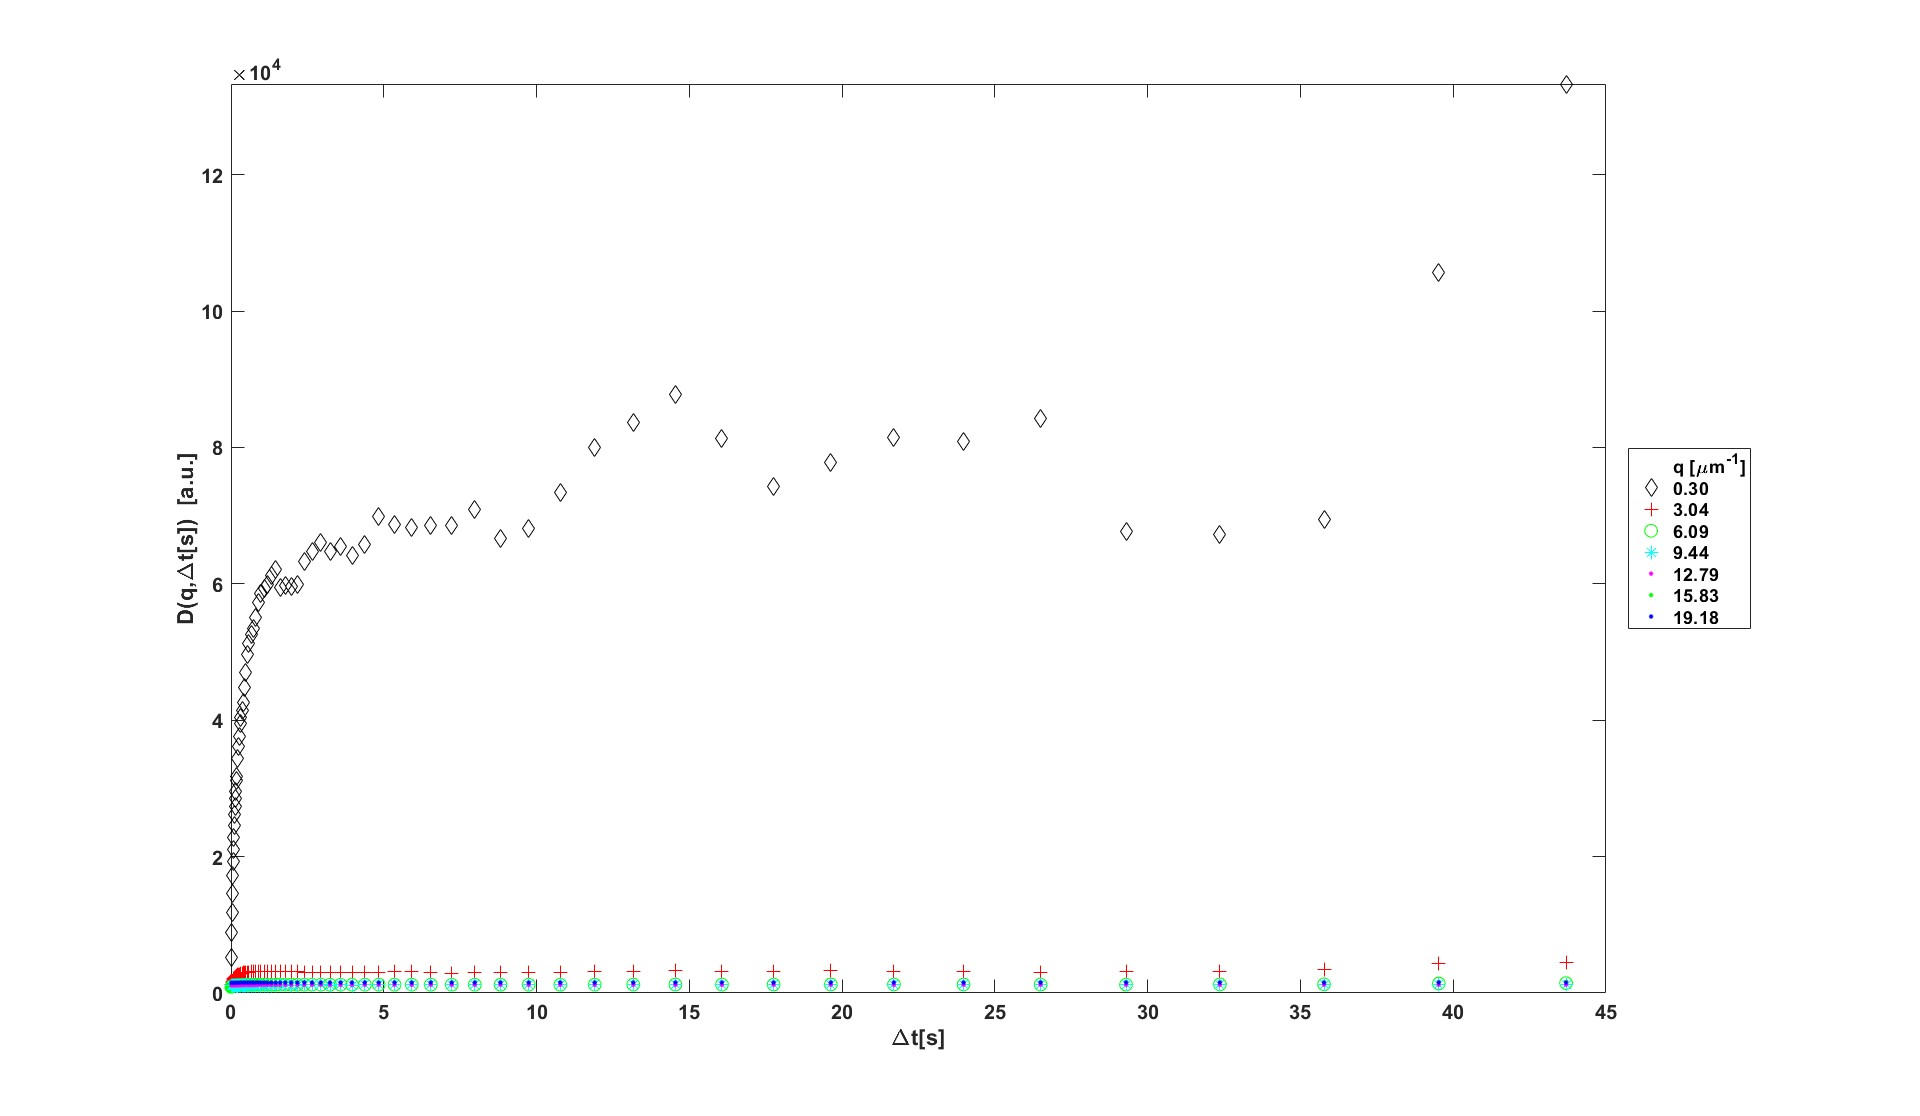
\includegraphics[width = \textwidth]{Bilder/Auswertung/DDM/d vs detat.jpg}
    \caption{The calculated dynamic structure function $D(q_x,q_y,\Delta t)$ is plotted against $\Delta t$ for selected $q$. For small $q$ an increasing $\Delta t$ leads to bigger noise and poor statistics.}
    \label{fig:DvsDeltat}
\end{figure}

As the dynamic structure function is expected to follow eq.~\ref{eq:21.3}, a fit was made, obtaining $A(q)$, $B(q)$ and $\tau (q)$. Eq.~\ref{eq:21.4} states 
\begin{equation}
    \tau (q) \propto q^{-2}
\end{equation}
and therefore the log-log-plot of $\tau (q)$ against $q$ should be a straight line with slope \num{-2}. As can be seen in fig.~\ref{fig:tauvsQ}, this is not the case for too small or too big $q$. Consequently a range for $q$ for the application of the fit of eq.~\ref{eq:21.4} was set. In this way, for each dataset a value for $D_m$ was obtained. As for every configuration of the setup five measurements were done, the $D_m$ were averaged afterwards. The results are stated in tab.~\ref{tab:Dm}.

\begin{figure}[ht]
    \centering
    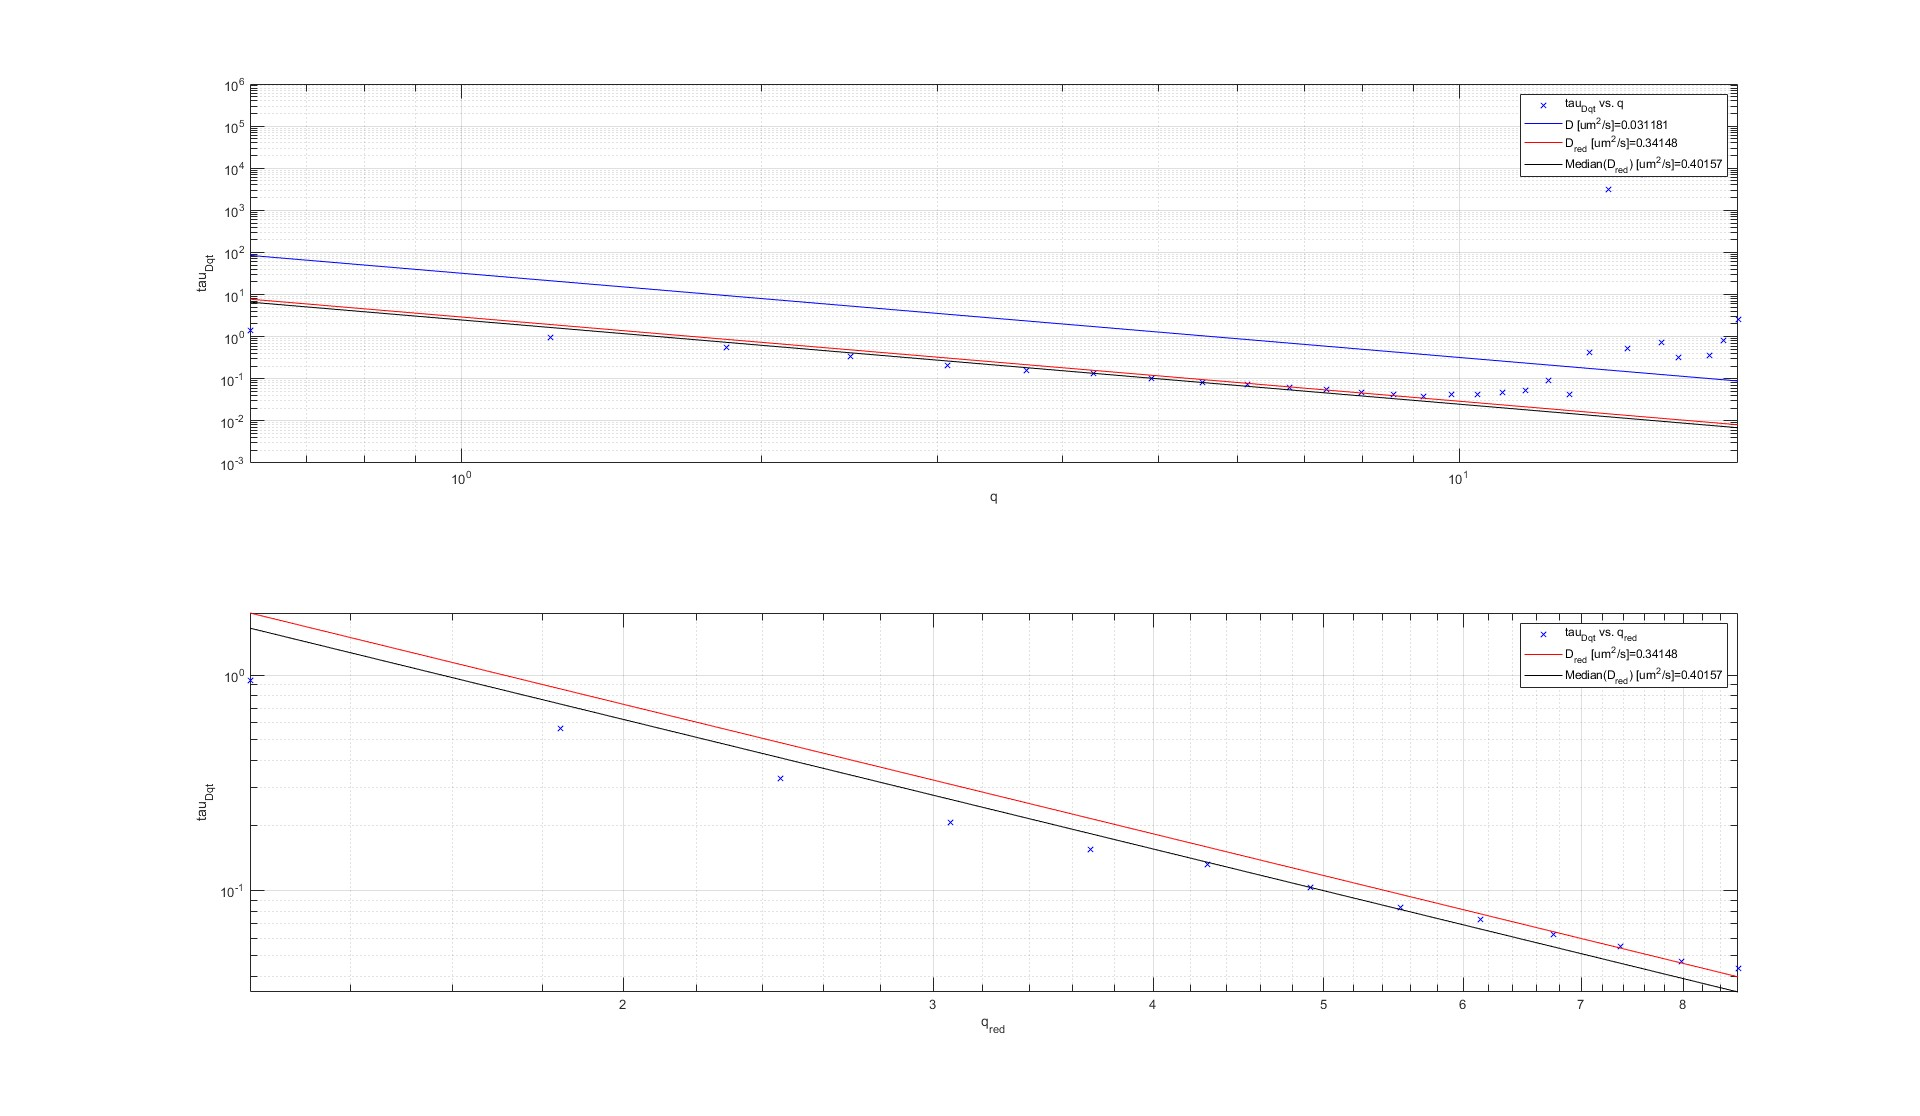
\includegraphics[width = \textwidth]{Bilder/Auswertung/DDM/tauvsQ.jpg}
    \caption{The values for $\tau (q)$ obtained from the fits were plotted against $q$ (upper plot). Too small and too big $q$ do not follow eq.~\ref{eq:21.4} and therefore lead to a wrong value for $D_m$ (fit in blue). Cosequently, the fit is only applied to a manually defined reduced $q$ space (lower plot and fits in red and black).}
    \label{fig:tauvsQ}
\end{figure}

\begin{table}
    \centering
    \begin{tabular}{c c c | c c}
        \toprule
        binning & ROI size / px & pinhole & $D_m$ / \si{\micro\meter^2 \per\second} & range for $q$ / \si{\per\micro\meter}\\
        \midrule
        none & 256x256 & none & \num{1.7 \pm 0.4} & 1-4\\
        none & 256x256 & half open & \num{1.7 \pm 0.7} & 1-3\\
        none & 256x256 & closed & \num{1.6 \pm 0.4} & 1-4\\
        \midrule
        none & 128x128 & none & \num{1.8 \pm 0.6} & 1-3.5\\
        none & 128x128 & half open & \num{1.7 \pm 0.9} & 1-4\\
        none & 128x128 & closed & \num{2.2 \pm 0.2} & 1-4\\
        \midrule
        2x2 & 128x128 & none & \num{0.56 \pm 0.10} & 1-8\\
        2x2 & 128x128 & half open & \num{0.86 \pm 0.11} & 1-5\\
        2x2 & 128x128 & closed & \num{0.49 \pm 0.12} & 1-9\\
        \midrule
        2x2 & 64x64 & none & \num{0.63 \pm 0.15} & 1-7\\
        2x2 & 64x64 & half open & \num{0.7 \pm 0.3} & 1-5\\
        2x2 & 64x64 & closed & \num{0.55 \pm 0.09} & 1-7.5\\
        \midrule
        4x4 & 64x64 & none & \num{0.15 \pm 0.03} & 4-10\\
        4x4 & 64x64 & half open & \num{0.15 \pm 0.03} & 3.5-10\\
        4x4 & 64x64 & closed & \num{0.11 \pm 0.03} & 3-10\\
        \bottomrule
    \end{tabular}
    \caption{Calculated averaged values of $D_m$ for each setting. The selected range of $q$ can differ slightly throughout the single measurements of a setup. }
    \label{tab:Dm}
\end{table}

When looking at the selected $q$ ranges, it can be seen that for the 4x4 binning the resolution for small $q$ gets worse in comparison to smaller binning. This fulfills our expectations since due to the binning, more pixels are summarized to one. Therefore, the minimum evaluation length in our ROI increases and the resolution for small $q$ decreases (see also sec.~\ref{sec:qSpace}). However, we would also expect a smaller resolution for big $q$ with an decreasing ROI size, following the same argument. This we could not observe. In fact, the resoultion even increases and is best for the smallest ROI size (64x64 px). This might be due to a better measuring procedure after having done some measurements already. \\
We also observe in general smaller uncertainties and better fits for the closed aperture. This is expectable, since ,as shown in sec.~\ref{sec:LightSheet}, the thickness of the lightsheet decreases with the beam diameter. \\
Within a certain setup, the calculated values are more or less the same within the uncertainties. However, a change in setup leads to a different obtained $D_m$ value. This is suprising, since the probe did not change. Therefore, we assume, that binning and the ROI size has an effect on the measurement quality. To verify our calculated values, the theoretical value shall be estimated. As we are at diffusie timescales, the Stokes Einstein equation can be used, which proposes a diffusion constant of 
\begin{equation}
    D_{SE} = \frac{k_BT}{6 \pi \eta R_0}
\end{equation}
with the dynamic viscosity $\eta$ and the radius of the particle $R_0$. $\eta$ of the \SI{1}{\percent}wt agarose solution depends on various parameters, such as temperature, solvent properties etc. However, for our estimation, we assume $\eta = $\SI{0.01}{\pascal\second}. Further, in this experiment, $T=$\SI{300}{\kelvin} and $R_0=$\SI{100}{\nano\meter}. This leads to a theoretical value of 
\begin{equation}
    D_{SE} = \SI{0.22}{\micro\meter^2 \per\second}.
\end{equation}

This value corresponds best to the values with the maximum binning and the minimum ROI size in our measurement. This is surpising since we expect binning to decrease the measurement accuracy because the information of several pixels get summarized in only a single one, especially since the pixelsize is $d_{px} = $\SI{162.5}{\nano\meter} and therefore in the size range of the particles themselves. Additional binning therefore should not be able to sufficiently track the diffusion of the particles. Also the decrease in measurement area should lead to a maximum equal good result, since less information is gathered. The simplifications made (no flow present, 2d analysis of 3d diffusion) shlould not be an explanation for this discrepancy since those all overestimate the diffusion and therefore corrections would only increase the difference between expected and calculated values. We hence suppose that the error might be in the estimation of the theoretical value of $D_{SE}$ as especially the value for $\eta$ is quite uncertain, $D_{SE}$ may also vary in one order of magnitude which would lead to a support of the values of the non binned, big ROI sized setup.




    % 5.Kapitel Fazit
    %Matteo Kumar - Leonard Schatt
% Fortgeschrittenes Physikalisches Praktikum

% 5. Kapitel Einleitung

\chapter{Fazit}
\label{chap:fazit}




    % Matteo Kumar - Leonard Schatt
% Physikalisches Praktikum

% Anhang

\appendix
\chapter{Appendix}
% Text


    % Literatur
    \bibliographystyle{Auswertung.bst}
    \nocite{*}
    \bibliography{Auswertung.bib}

\end{document}